% Template for ISBI paper; to be used with:
%          spconf.sty  - ICASSP/ICIP LaTeX style file, and
%          IEEEbib.bst - IEEE bibliography style file.
% --------------------------------------------------------------------------
\documentclass{article}
\pdfoutput=1
\usepackage{spconf}
\usepackage{amsmath}
\usepackage{graphicx}
\usepackage{algorithmic}
\usepackage{multirow}
\usepackage{algorithm}
\usepackage{color}
% \usepackage{endnotes}
\usepackage{enotez}
\let\footnote=\endnote
\usepackage{tablefootnote}

% It's fine to compress itemized lists if you used them in the
% manuscript
\usepackage{enumitem}
\setlist{nosep, leftmargin=14pt}

\usepackage{mwe} % to get dummy images

% Example definitions.
% --------------------
\def\x{{\mathbf x}}
\def\L{{\cal L}}

\let\footnote=\endnote
\newcommand{\soumya}[1]{\textcolor{red}{#1}}
\newcommand{\update}[1]{\textcolor{black}{#1}}
\newcommand{\final}[1]{\textcolor{black}{#1}}

\newcommand{\rpm}{\raisebox{.2ex}{$\scriptstyle\pm$}}

% Title.
% ------
% \title{OsteophyteNet: Automated Osteophyte Identification in Spine Radiographs}
\title{Spinal Osteophyte Detection via Robust Patch Extraction on Minimally Annotated X-rays}
%
% Single address.
% ---------------
%
% For example:
% ------------
%\address{School\\
%	Department\\
%	Address}
%
% Two addresses (uncomment and modify for two-address case).
% ----------------------------------------------------------
%\twoauthors
%  {A. Author-one, B. Author-two\sthanks{Some author footnote.}}
%	{School A-B\\
%	Department A-B\\
%	Address A-B}
%  {C. Author-three, D. Author-four\sthanks{The fourth author performed the work
%	while at ...}}
%	{School C-D\\
%	Department C-D\\
%	Address C-D}
%
% More than two addresses
% -----------------------
% \name{Author Name$^{\star \dagger}$ \qquad Author Name$^{\star}$ \qquad Author Name$^{\dagger}$}
%
% \address{$^{\star}$ Affiliation Number One \\
%     $^{\dagger}$}Affiliation Number Two
%
\name{ Soumya Snigdha Kundu$^{\star}$\thanks{*S.S.K carried out the work as a part of the Big Data Institute Summer Internship Programme at the University of Oxford.} \qquad Yuanhan Mo$^{\dagger}$ \qquad Nicharee Srikijkasemwat$^{\star\star}$ \qquad Bart\l omiej W. Papie\.z $^{\dagger}$}

\address{$^{\star}$ Department of Surgical \& Interventional Engineering, King's College London, London, UK \\
$^{\star\star}$ Department of Engineering Science, University of Oxford, Oxford, UK \\
    $^{\dagger}$ Big Data Institute, University of Oxford, Oxford, UK } 
\begin{document}
%\ninept
%
\maketitle

%%%%%%%%%%%%%%%%%%%%%%%%%%%%%%
% I have removed densenet and resnet citations. Is that okay? It was crossing 6 pages. Every other citation is imoprtant i feel.
%%%%%%%%%%%%%%%%%%%%%%%%%%%%%%


\begin{abstract}
% Osteophytes are small and often elusive bone growths which strongly associate with the development and progression of arthritis.
The development and progression of arthritis is strongly associated with osteophytes, which are small and  elusive bone growths. This paper presents one of the first efforts towards automated spinal osteophyte detection in spinal X-rays.
% By utilizing a specialized patch generation process called SegPatch, which encompasses deep learning-driven vertebrae segmentation and the enlargement of mask outlines, we have attained a patch classification precision rate of 84\%.
A novel automated patch extraction process, called SegPatch, has been proposed based on deep learning-driven vertebrae segmentation and the enlargement of mask contours. 
A final patch classification accuracy of 84.5\% is secured, surpassing a baseline tiling-based patch generation technique by 9.5\%. 
This demonstrates that even with limited annotations, SegPatch can deliver superior performance for detection of tiny structures such as osteophytes.
The proposed approach has potential to assist clinicians in expediting the process of manually identifying osteophytes in spinal X-ray.
\end{abstract}
%
\begin{keywords}
Keypoint Identification, Osteophyte Detection, Patch Extraction.
\end{keywords}
%

\section{Introduction}
\label{sec:intro}
One of the features observed in osteoarthritis (OA) \cite{van2007osteophytes} are osteophytes which are  fibrocartilage-capped  bony outgrowths. They play a strong role in determining the severity and progression of OA. Osteophytes also cause problems by impinging nerves such as spinal roots \cite{jones2012l5} and pose significant issues in many other spinal diseases.
\par
The manual identification of osteophytes has been generally done using
Magnetic Resonance Imaging (MRI) \cite{tozawa2021possible}. In contrast, the use of X-rays has been limited due to the challenges associated with the quality and 2D nature of conventional radiography. 
Automated detection of spinal osteophytes has also been explored. 
% Wang et al \cite{wang2016detection} presented a bottom-up approach to generate features for classification using a region-based convolutional neural network with unwrapped cortical shell maps from F-NaF positron emission tomography and computed tomography scans of the vertebral bodies of the thoracic and lumbar spine. 
Wang et al. \cite{wang2016detection} extracted region proposals and classified them from unwrapped cortical shell maps in Positron Emission Tomography and Computed Tomography scans of the vertebral bodies of the thoracic and lumbar spine. 
They achieved 85\% sensitivity at 2 false positive detections per patient. 

Automated approaches to detect osteophytes in other parts of the body has been proposed as well. 
Ebsim et al., \cite{ebsim2022automatic} identified hip osteophytes in dual-energy X-ray absorptiometry by segmenting the osteophyte regions using U-Net \cite{ronneberger2015u} and manual cropping (to highlight the area of interest). 
Banerjee et al \cite{banerjee2011osteophyte} identified hand osteophytes in X-rays through cellular neural networks (neural networks where communication is allowed only between neighboring units). They automated the ground truth acquisition but they lacked any involvement  from an actual clinical representative throughout the acquisition process. 
\final{The VinDr-SpineXR study \cite{nguyen2021vindr} provides an extensive dataset with baseline results on multiple spinal diseases, including osteophytes. The poor results (and trend of increasing performance with increasing label size) match with our detection findings in sec 5.3.}
% Oka et al. \cite{oka2010normal} established normal and threshold values of radiographic parameters for knee OA using the knee osteoarthritis computer-aided diagnosis measuring system on a large-scale population-based cohort.  

% \begin{figure}
%     \centering
%     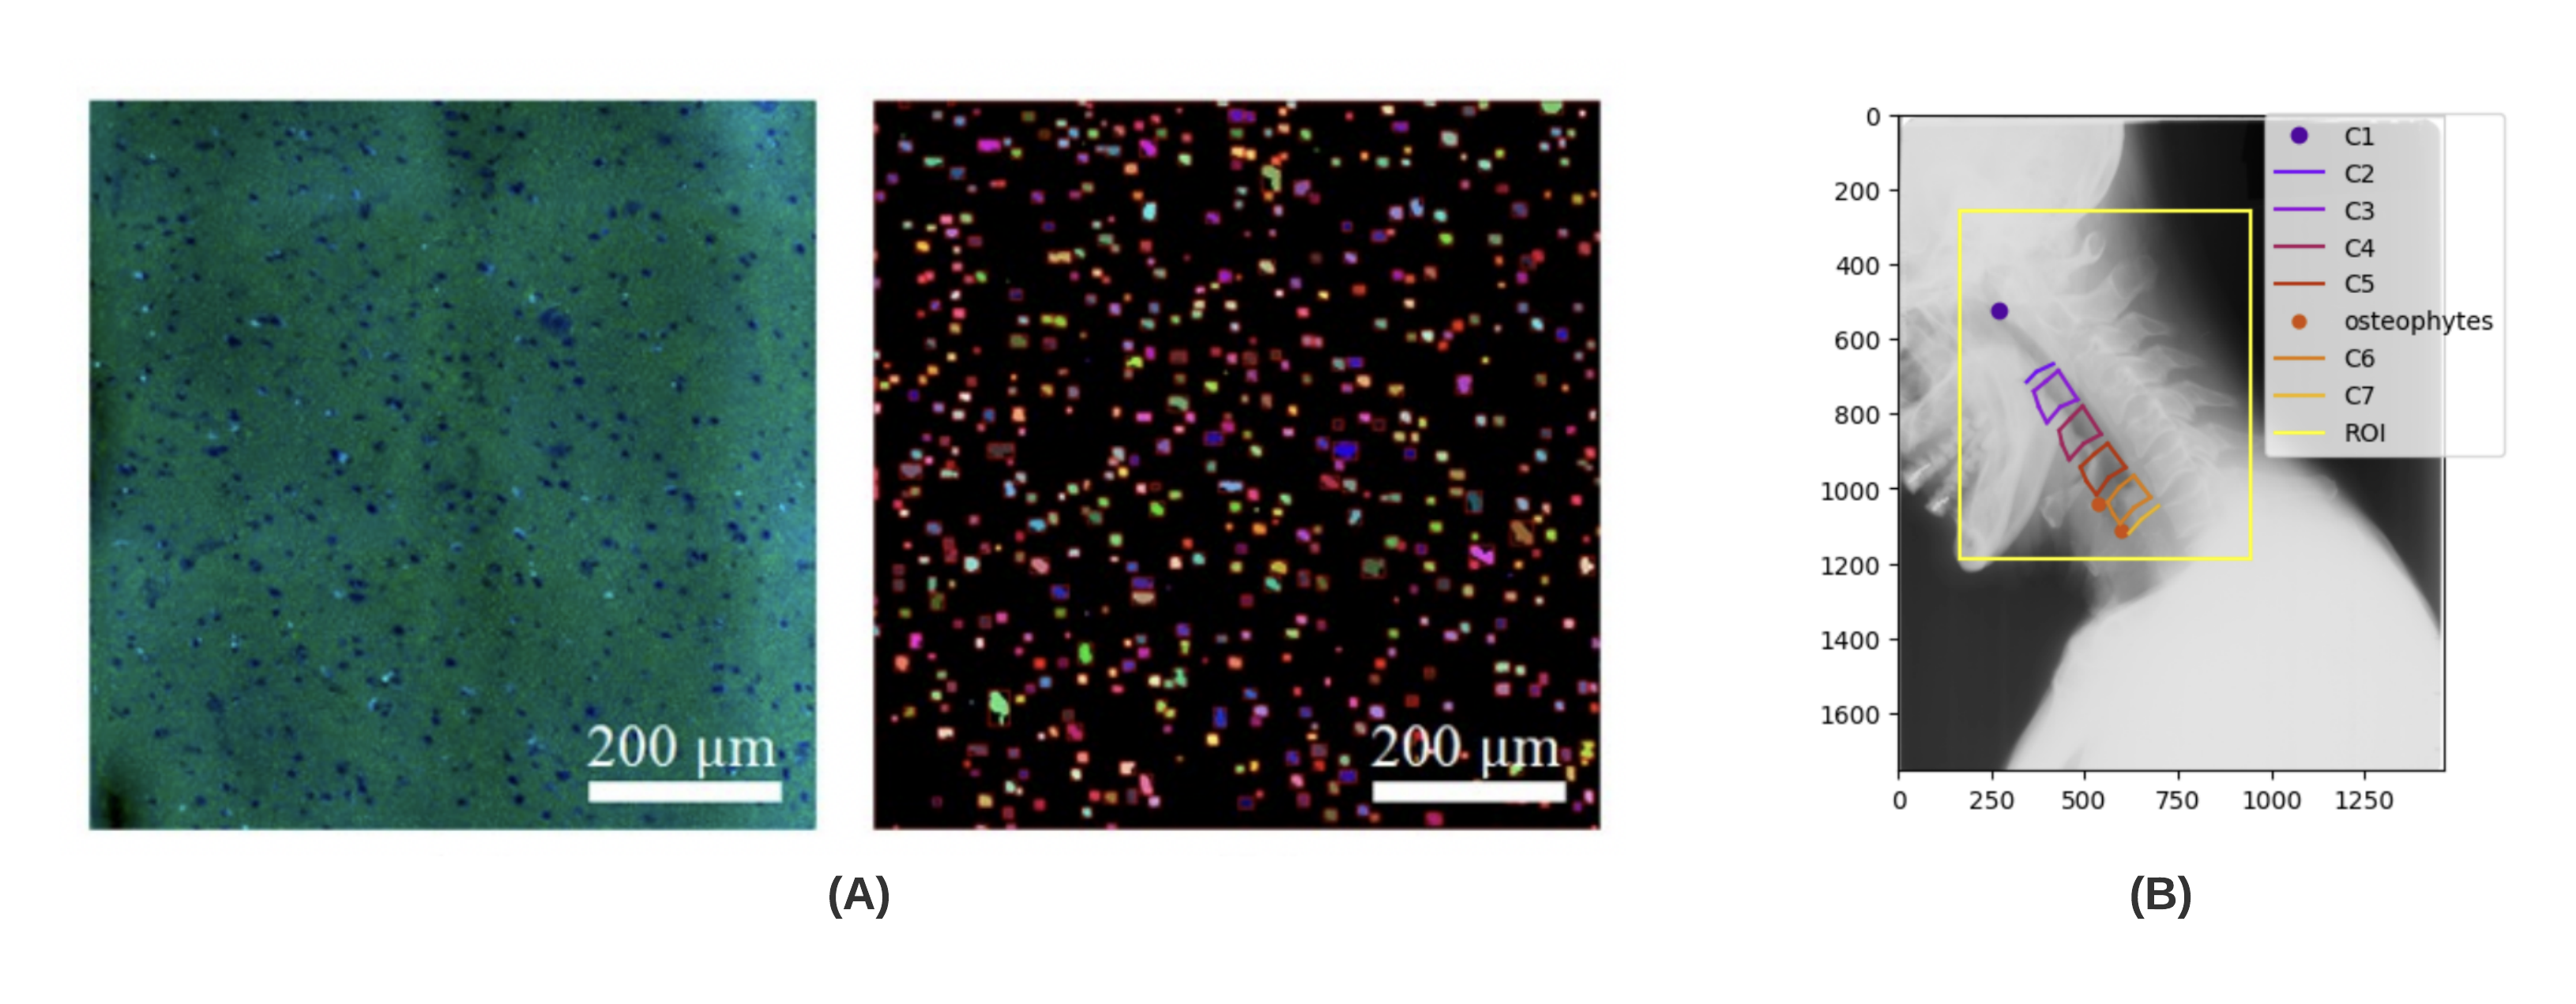
\includegraphics[width=0.36\textwidth]{images/annotation.png}
%     \caption{Examples of annotation for medical key-point detection. (A) Annotations for cell counting (taken from \cite{zhang2021automatic}). (B) Example Annotation from NHANESII$^3$.}
%     \label{fig:nhanes-osteophyte-label}
% \end{figure}


\begin{figure}
    \centering
    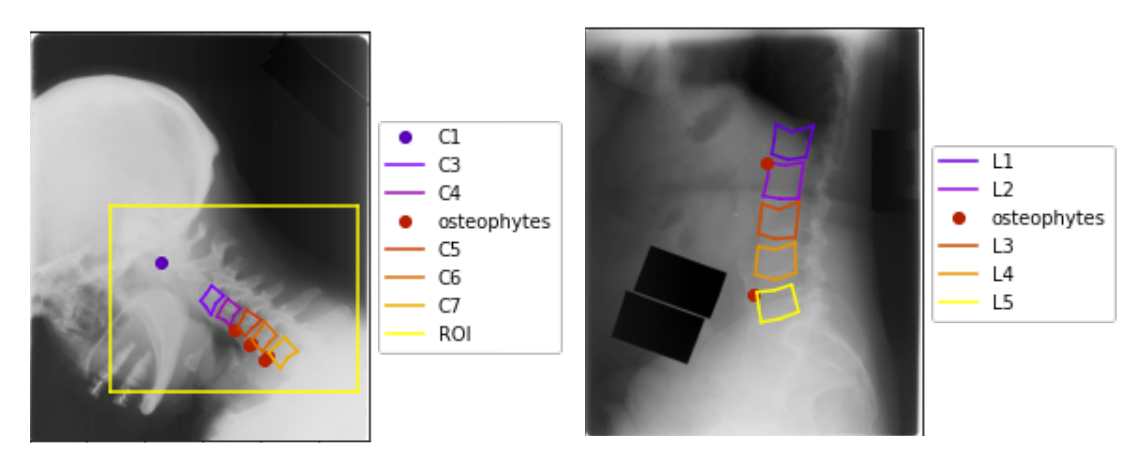
\includegraphics[width=0.48\textwidth]{images/Annotated_NHANES.png}
    \caption{Example of annotations for cervical (left) and lumbar (right) X-ray scan available from NHANESII$^2$ data set.}
    \label{fig:nhanes-osteophyte-label}
\end{figure}

The number and size of the osteophytes could be seen as an estimate of the OA progress. Clinical experts' annotations are time-consuming and expensive while being prone to errors (i.e. inter- and intra-reader variability). Especially for tiny structures such as osteophytes. To the best of our knowledge, there has been no automated method for spinal osteophyte detection for spinal X-rays. 

\begin{figure*}[t]
    \centering
    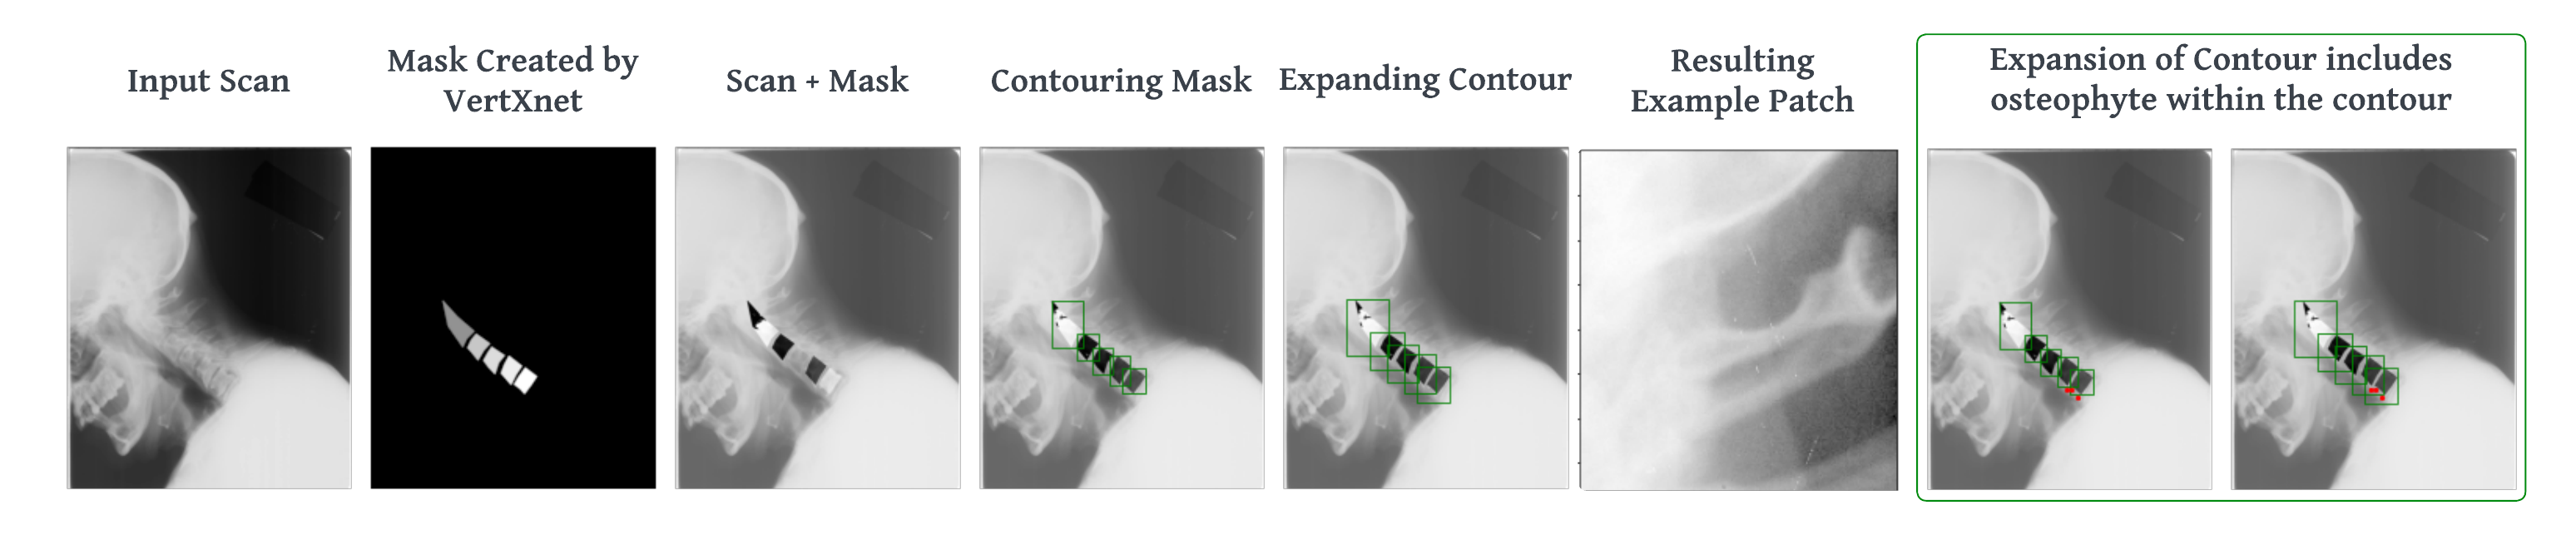
\includegraphics[width=1\textwidth]{images/Pipe-SegPatch.png}
    \caption{A representation of the SegPatch pipeline with a resulting patch. The green box highlights the necessity to expand contours to fully encompass the osteophytes within the boundary. Red dots denote the osteophytes.}
    \label{fig:pipeline}
\end{figure*}

% Alongside the immediate clinical advantages, key-point detection in medical images has largely been an unsolved problem. 
% While literature exists for problems such as cell counting \cite{morelli2021automating, kataras2023acct, zhang2021automatic}, almost all papers consider key-points which are clusters of pixels rather than single pixel values (ref: Fig \ref{fig:nhanes-osteophyte-label}). 
% This makes the problem significantly less complex. 
% In general real-world applications, such as pose estimation \cite{8455796}, priors, and context (such as the location and correlation between different limbs of a person) can be utilized. 
% \soumya{In osteophyte detection, the overall region of occurrence tends to be consistent, akin to many medical conditions. However, the specific localization of these occurrences exhibits a high degree of randomness.}



% This paper presents OsteophyteNet, a novel deep learning approach to detect osteophytes of the spine from cervical and lumbar radiographs. 
% First, a custom patching strategy, termed SegPatch, based on vertebrae segmentation and expansive contouring was proposed and combined with a fine-tuned classifier network to perform the detection of osteophytes. 
% Furthermore, the work delves into potential avenues for enhancement and offers key pointers for future methods of osteophyte identification.
Our contributions are as follows - We have developed a method to automatically identify osteophytes from conventional spinal radiography. First, we proposed a robust mechanism SegPatch, to extract patches from the spinal X-ray images through a deep-learning based vertebrae body segmentation approach \cite{chen2023vertxnet}.

Unlike the standard tiling approach, the newly proposed patching generates patches that are associated with potential locations of the osteophytes. Thereafter, we trained multiple neural network models for classification. 
Our framework was evaluated using the publicly available spine X-ray data set NHANESII. We compared SegPatch with the baseline tiling method. The results show the significant advantage of using SegPatch.



%\begin{itemize}
 %   \item A crucial advancement in the detection of osteophytes in X-ray images, particularly an area with limited prior research. 
%    Identifying osteophytes in Spinal X-rays, rather than depending on MRIs or multi-modal approaches, could greatly streamline the diagnosis process.
%    \item The SegPatch stands out as one of the few methods designed to automate the identification of key regions of interest, specifically for the detection of osteophytes.
%    \item Use of limited annotations and showcasing interpretability. This is in contrast to many other medical key-point detection literature that necessitates extensive annotation areas \cite{kataras2023acct} or wide segmentation ground truths for osteophyte detection based on segmentation \cite{ebsim2022automatic}.
    % \item Analysis of key areas of enhancements for future methods of osteophyte identification.
%\end{itemize}


\section{Data}
The method was developed based on the publicly available data set\footnote{This research study was conducted retrospectively using human subject data made available in open access$^2$. Ethical approval was not required as confirmed by the license attached with the open access data.} collected via the Second National Health and Nutrition Examination Survey (NHANES II)\footnote{Dataset information can be found here: \newline
https://data.lhncbc.nlm.nih.gov/public/NHANES/X-rays/README.html .} conducted by the National Center for Health Statistics
% NCHS 
during the years 1976-1980. 
The data encompasses digitized versions of the 17100 X-ray films. 9670 were cervical (of the size 1462 x 1755) and 7430 lumbar (of the size 2048 x 2487). 
However, only 241 cervical and 232 lumbar X-ray images were annotated for pixel coordinates indicating the presence of osteophytes. 
Each vertebrae was delineated using six pixel points.
A 75:25 split was employed for training and testing data.
The exemplar radiographs and the associated annotations have been shown in Fig.~\ref{fig:nhanes-osteophyte-label}.

% \begin{figure}
%     \centering
%     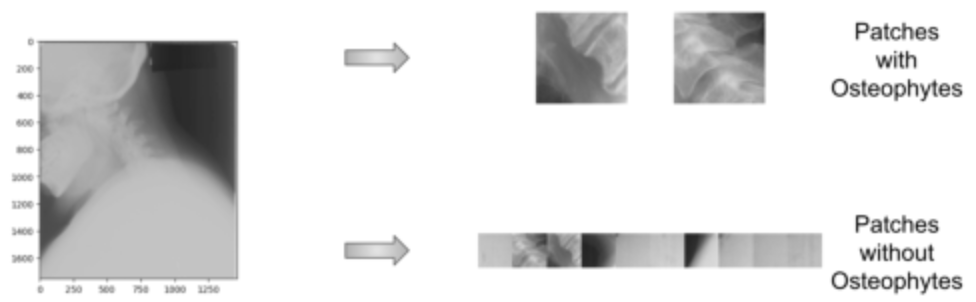
\includegraphics[width=0.4\textwidth]{images/tilingbw.png}
%     \caption{Example of created (labelled) patches via Tiling (for Cervical scan).}
%     \label{fig:enter-label}
% \end{figure}


\section{Methodologies}
%As seen from Fig \ref{fig:nhanes-osteophyte-label}, providing an area of interest to the clinician can provide a similar aid in diagnostic accuracy.
Given the challenges associated with the detection of the miniscule osteophytes, the main goal of this research was to create a technique that could ascertain whether a particular image patch contained an osteophyte.
As seen in Fig.~\ref{fig:nhanes-osteophyte-label}, osteophytes generally tend to occur on the corners of the vertebrae. 
Based on this observation we developed a pipeline to extract several patches from high-resolution radiographs (Sec. \ref{sec:patch_creation}) and classify those patches for the presence of an osteophyte (Sec. \ref{sec:patch_classification}). 
Therefore, we set the hypothesis that if a patch is classified as "present", then either of the two corners of the vertebrae will have an osteophyte.
If the patch contains only one corner then it is bound to have a single osteophyte. 

For an qualitative evaluation, \final{the explainability of the classifier was tested via class activation map generation method SS-CAM \cite{wang2020ss}, to} understand and verify the focus of the classifier.
%Hence, we primarily posed a problem of patch classification. 

% \begin{figure}
%     \centering
%     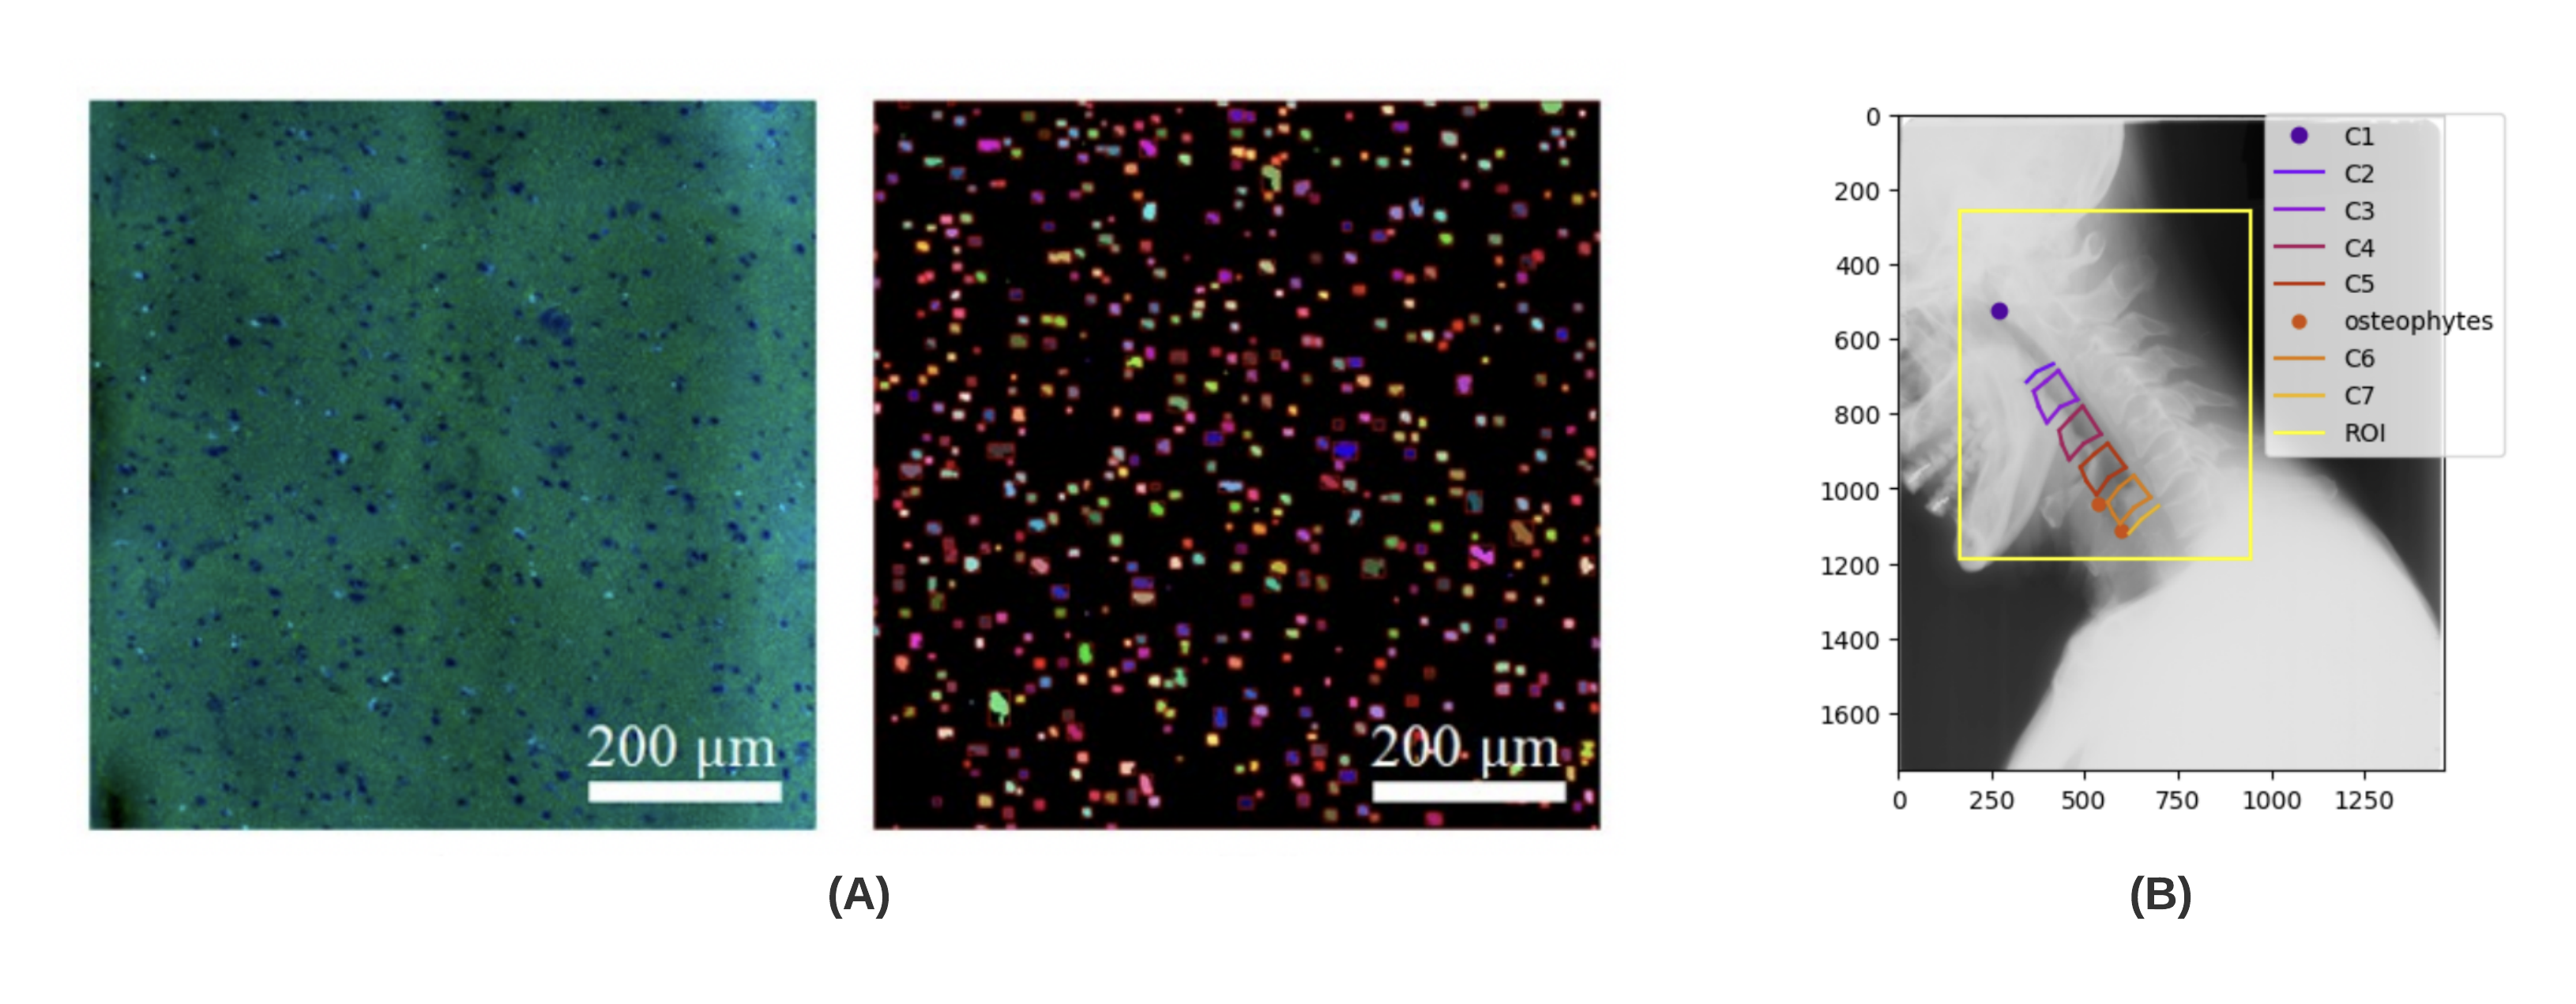
\includegraphics[width=0.35\textwidth]{images/annotation.png}
%     \caption{Examples of annotation for medical key-point detection. (A) Annoations for cell counting (taken from \cite{zhang2021automatic}). (B) Example Annotation$^3$.}
%     \label{fig:nhanes-osteophyte-label}
% \end{figure}

\subsection{Robust Patch Creation}
\label{sec:patch_creation}
Two methods of patch creation were investigated in this study.
\subsubsection{Tiling}
The tiling approach was inspired from Ozge et al.~\cite{ozge2019power}. The authors proposed it for a detection task in high-resolution pedestrian and vehicle images. Here, tiling is used as an image pre-processing step to split the image into equal-sized non-overlapping patches and label them based on whether a patch contained an annotation - indicating the presence of an osteophyte. 
To ensure the corner regions were not split amongst patches, the annotations were considered as boxes.
% The default patch size of 224x224 was used to avoid resizing of the X-ray image as resizing could lead to blur the appearance of the osteophyte in the image. 
% As the content of the patches depended on the box size, different box sizes were considered, which varied which patch contained the actual annotation. 
The tiling approach generated a highly imbalanced set of patches. The number of patches containing osteophytes amounted to 1453 ($<$ 5\%). Those without equalled to 32160. The boxes used as annotations were also used as the ground truth bounding boxes for the detection task in section \ref{detection}.

\subsubsection{SegPatch: Segmentation-driven Patch Extraction}
% There were a number of challenges associated with the tiling approach along with the high class imbalance. 
% % As mentioned above, it was dependent on the size of the bounding box considered. 
% The tiling involved the entire scan, while focusing only on the vertebrae region could immediately reduce the noise faced by the classifier. 
% Lastly, if there were no annotations, there were no patches formed in the tiling. 
% Hence, we needed to account for potential healthy cases as well. 
The main challenge in tiling was the significant class imbalance generated by considering the complete scan. Any approach which could focus on the vertebrae region alone, would potentially improve performance as the amount of noise seen by the classifier would reduce.
Therefore, a custom patch-generating method called SegPatch was devised to overcome the above limitations.

% \begin{itemize}
%     \item To reduce the number of patches in order to solve the class imbalance issue and avoid bias.
%     \item Become bounding box size independent for a potential improved detection network.
%     \item Ensure only relevant patches (that is every patch containing a vertebrae) is considered.
%     \item Patches should be spine curvature and artifact invariant. Should also generate in abscence of osteophyte.
% \end{itemize}

% \begin{table}
% \caption{Classification results for Tiling}
% \label{tiling}
% \centering
% \resizebox{0.3\textwidth}{!}{%
% \begin{tabular}{|c|c|c|}
% \hline
% \textbf{\begin{tabular}[c]{@{}c@{}}Patch \\ Size\end{tabular}} & \textbf{\begin{tabular}[c]{@{}c@{}}Accuracy \% \\ (Without PreText Task)\end{tabular}} & \textbf{\begin{tabular}[c]{@{}c@{}}Accuracy \% \\ (With PreText Task)\end{tabular}} \\ \hline
% 10                                                             & 71 $\rpm$ 1                                                                                  & 71.5 $\rpm$ 0.5                                                                               \\ \hline
% 18                                                             & 69 $\rpm$ 1                                                                                  & 71 $\rpm$ 1                                                                               \\ \hline
% 36                                                             & 71 $\rpm$ 1                                                                                 & 72 $\rpm$ 1                                                                              \\ \hline
% 54                                                             & 73 $\rpm$ 2                                                                                  & 67 $\rpm$ 1                                                                               \\ \hline
% \end{tabular}%
% }
% \end{table}

The SegPatch process begins by utilizing a vertebrae segmentation network VertXNet \cite{chen2023vertxnet} to localise the vertebrae in the scan. 
%This was done as it was the most efficient method to access the vertebrae locations. 
However, while the segmentation accounted for each vertebra in each image, it failed to encapsulate the osteophyte point locations (given as per the dataset). 
% Whether due to an algorithmic error or a labeling mistake, the frequent occurrence of osteophytes located outside the designated area was notable. 
This is most likely because the reader was asked to place the marker along the center of gravity for each vertebra.

Therefore, a simple contour of the vertebra  did not suffice. To account for \final{the inclusion of the osteophyte location into the final resulting patches}, another strategy was implemented consisting of expanding the formed contour. 
The majority of the osteophytes occurred on the left side of the vertebrae hence we first expanded the contour in the -X direction. To account for the curvature of the spines, we also expanded the contour in the +Y direction. This allowed for the gaps between the vertebrae to be covered. Different size of expansion was utilized for cervical and lumbar scans to account for the variation in vertebra sizes. SegPatch finally resulted in 1680 present patches and 1517 absent patches, which was more favourably distributed than the tiling method described above. The details and visual depiction are outlined in Fig.~\ref{fig:pipeline}. \final{A rigid rule and clinical prior based heuristic was used to expand the contour to prevent further processing of the image prior to being fed to the classifier.}

\begin{figure}
    \centering
    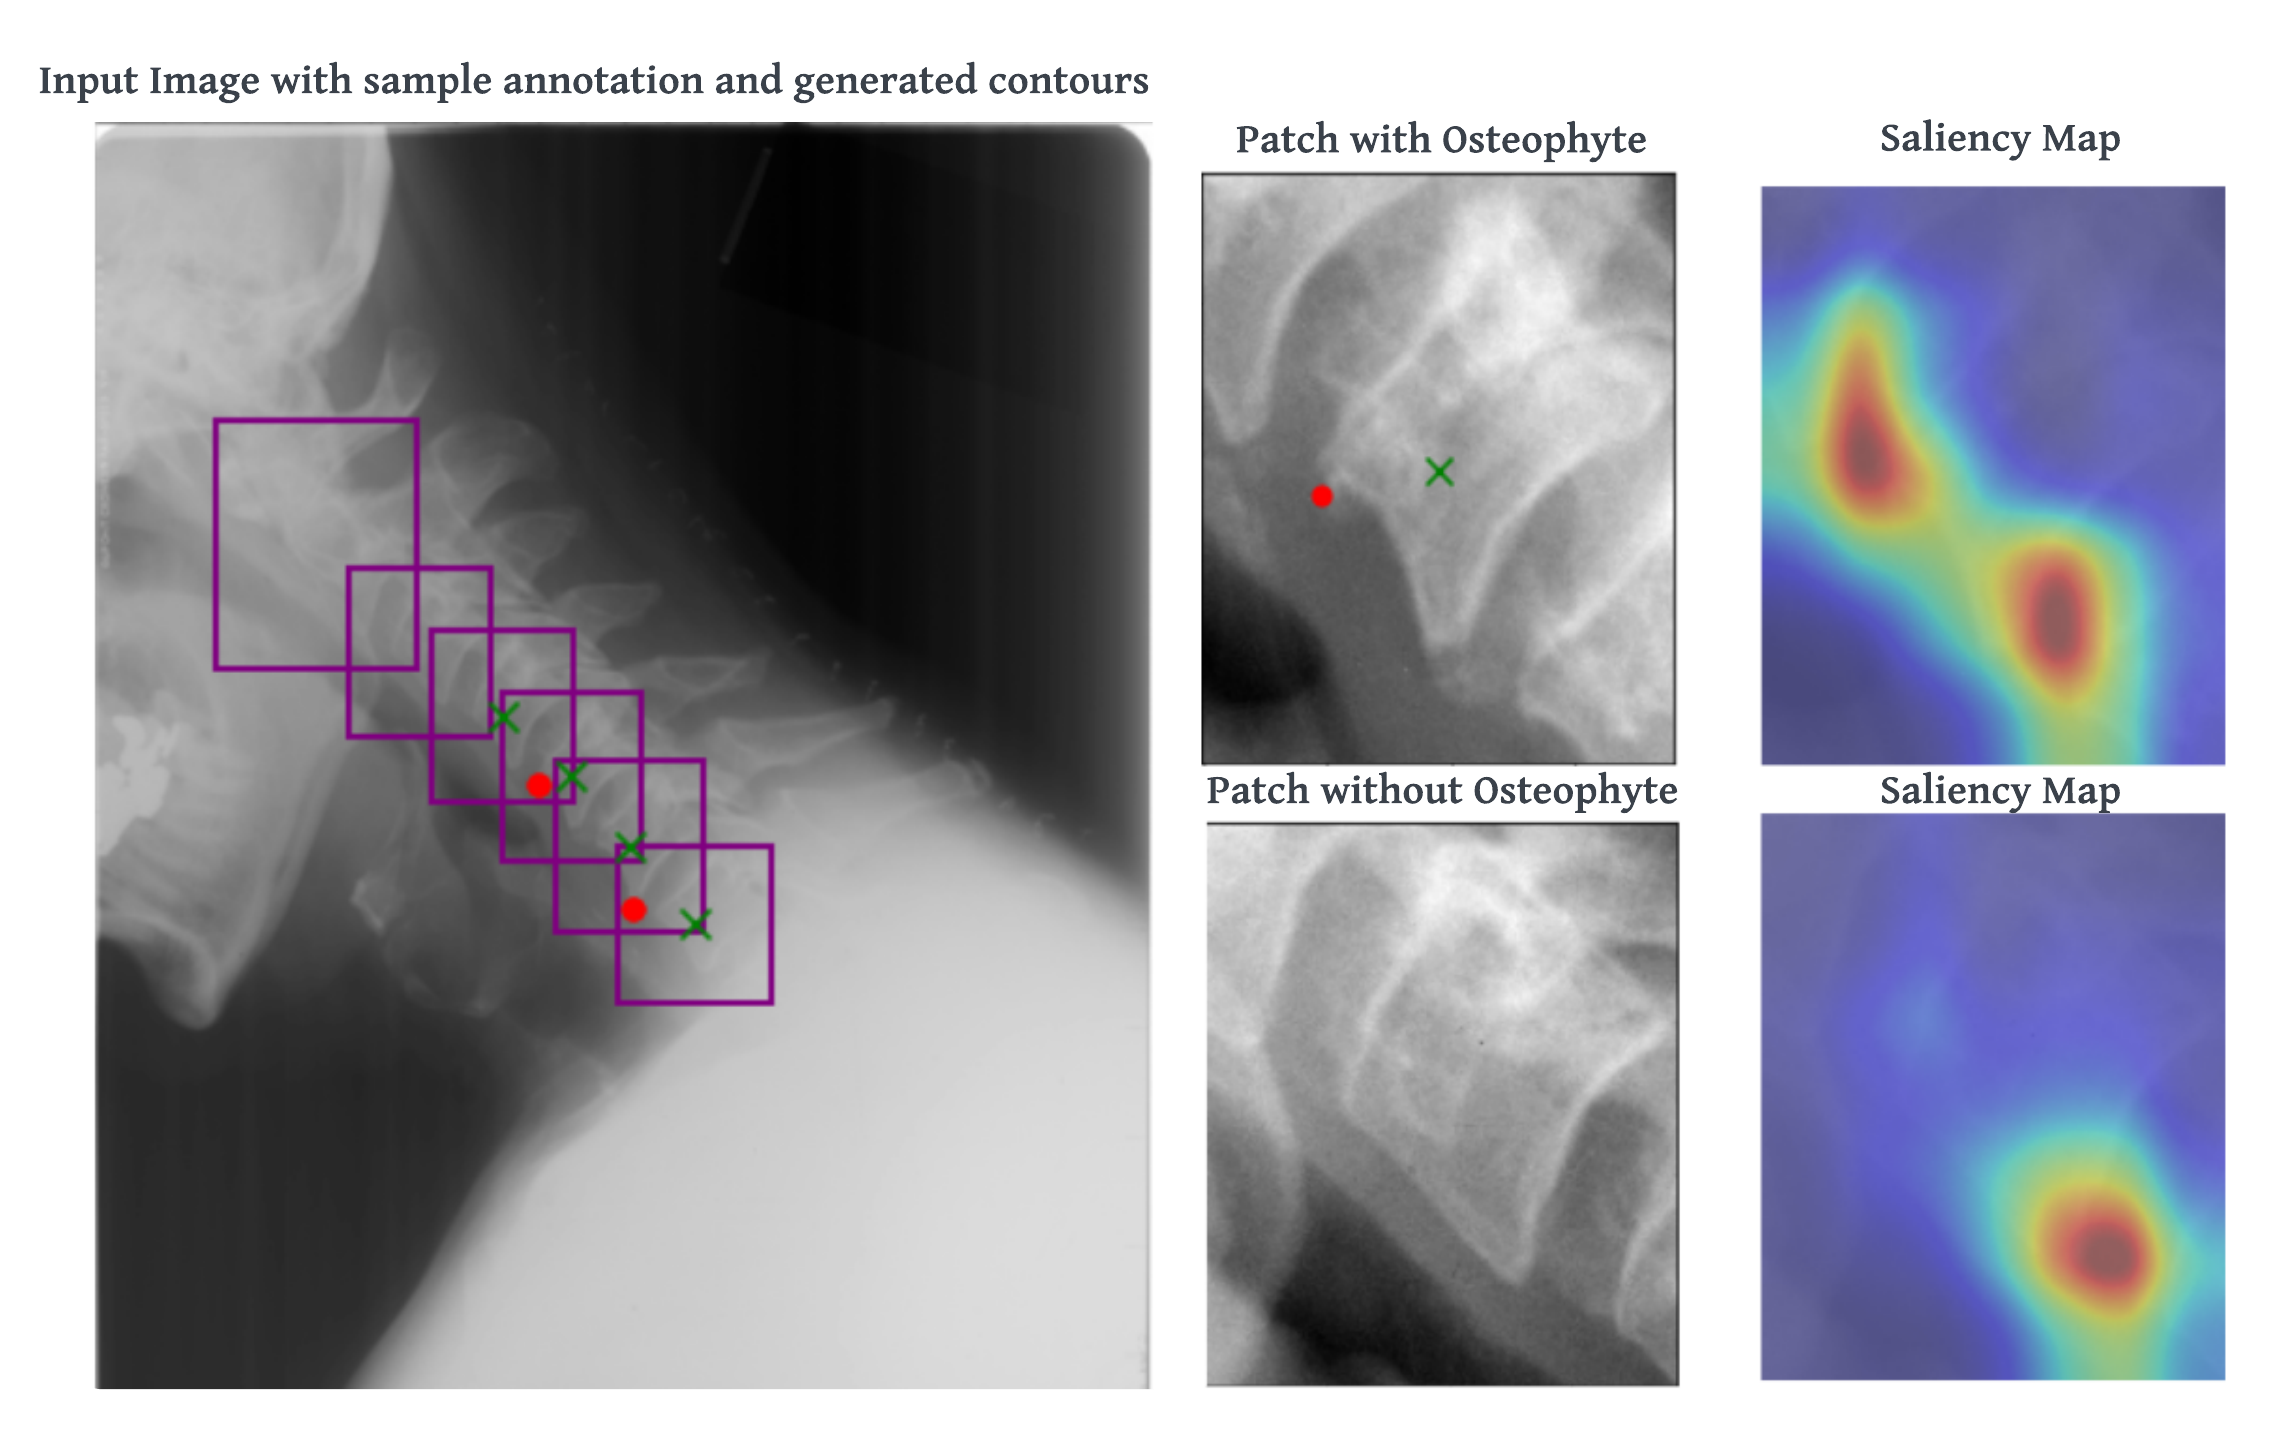
\includegraphics[width=0.48\textwidth]{Explainability_Example.png}
    \caption{Saliency results for a positive and a negative patch. Red dots: Osteophytes. Purple boxes: Contours.}
    \label{fig:Explainability}
\end{figure}

\subsection{Classification of Osteophytes}
\label{sec:patch_classification}
% In our experiments, DenseNet-121 produced the best score. 
% The highest performance was achieved with augmentations involving random rotation of up to 30 degrees and random histogram equalization (with variance of 0.5). 
% 32 batch size and ResNet-18 was used for tiling. 18 batch size and DenseNet-121 was used for SegPatch. The patches were resized to (244 x 224) in the case of SegPatch and the tiling limit was set to (244 x 224). 

% In both cases, a 75:25 split was used for training versus testing and a cross entropy loss along with Stochastic Gradient Descent. Tiling had the parameters of 0.01 learning rate and 0.7 momentum. SegPatch performed best with 0.002 learning rate and 0.09 momentum. With a step size of 7 and gamma value of 0.1 a a learning rate scheduler was used as well. Maximum results were achieved within 50 epochs in both cases.
Multiple state-of-the-art classifiers were tested including ResNet-18/50 and DenseNet-121/169, all pretrained on ImageNet.
Given the limited amount of annotated images, we employed data augmentation including random rotations (up to 30 degrees) and random histogram equalization (with a variance of 0.5). 
% The image patches were resized to (244 x 224) for SegPatch, and the tiling limit was set to (244 x 224).
The input dimensions for both strategies are the same. The image patches were resized to (244 x 224) for SegPatch, and the tiling limit was set to (244 x 224).
For both methods, the cross-entropy loss, and the Stochastic Gradient Descent were used. 
Tiling was fine-tuned with a learning rate of 0.01 and a momentum of 0.7, while SegPatch achieved optimal results with a learning rate of 0.002 and a momentum of 0.09.
Additionally, a learning rate scheduler with a step size of 7 and a gamma value of 0.1 was employed. Peak performance was reached at 50 epochs for both approaches.

% \begin{algorithm}[b]
% \caption{SegPatch}
% \begin{algorithmic}
% \STATE \textbf{Input}: Cervical or Lumbar X-ray
% \STATE \textbf{Output}: Classification of Patches

% \STATE \textbf{1:} Generate vertebrae masks via VertXNet \cite{chen2022vertxnet}.
% \STATE \textbf{2:} Generate contours of segmented masks.

% \FOR{each contour}
%     \STATE \textbf{3a:} Generate bounding box (bbox) over contours.
    
    
%     \STATE \textbf{3b:} Adjust bbox based on Lumbar or Cervical.
    
%     \STATE \textbf{3c:} Check presence of osteophyte within the bbox:

%     $x_{\text{min}} \leq \text{point}[x] \leq x_{\text{max}}$ and $y_{\text{min}} \leq \text{point}[y] \leq y_{\text{max}}$
    
%     \IF{Osteophyte is present: }
%         \STATE \textbf{3d:} Classify patch as present \textbf{else} absent.
%     \ENDIF

% \ENDFOR

% \end{algorithmic}
% \end{algorithm}

\section{Results}
% As seen from Table \ref{Segpatch_Scores}, tiling achieves an average test accuracy range of 74\% and SegPatch outperforms this by 9\% achieving an average score of 84\%. 
% % The training accuracy averaged around 80\% in the case of Tiling and 86\% in SegPatch which hints towards generalizability of both approaches. 
% The training accuracy averaged \update{to} 80\% in the case of Tiling and 86\% in SegPatch which hints towards generalizability of both approaches. \update{Further, from Fig. \ref{fig:pipeline}, it is quite interesting to see that in the present patch, the saliency is over the edges where the osteophyte is, but in the absent patch, it focuses on the edge, but not where the osteophyte is. This clearly depicts the model is looking at the edges and determining whether there is growth or not. Maps were created using SS-CAM \cite{wang2020ss}.}

% For the tiling approach, a batch size of 32 was utilized, and ResNet-18 was employed. 
% In the case of SegPatch, a batchsize if 18 was chosen, along with DenseNet-121 as the architecture. 
As indicated in Tab.~\ref{Segpatch_Scores}, the tiling method produced an average test accuracy of 75.4\%, whereas SegPatch surpasses this performance, achieving an average accuracy of 84.5\%. 

Furthermore, Fig.~\ref{fig:Explainability} reveals an interesting observation: in the present patch, the saliency maps generated using SS-CAM are predominantly concentrated over the edges where the osteophyte is present. In the absence of an osteophyte, it primarily focuses on the edge but not on the location of the osteophyte. This observation vividly illustrates that the model is discerning the edges and making determinations regarding the presence or absence of growth by looking specifically at the edges of the vertebrae.

% Please add the following required packages to your document preamble:
% \usepackage{multirow}
\begin{table}[]
\centering
\caption{Classification results for the proposed patching algorithms.}
\label{Segpatch_Scores}
\begin{tabular}{|lcccc|}
\hline
\multicolumn{1}{|c|}{\multirow{3}{*}{\textbf{Model}}} & \multicolumn{4}{c|}{\textbf{Accuracy Score}}                                                           \\ \cline{2-5} 
\multicolumn{1}{|c|}{}                                & \multicolumn{2}{c|}{\textbf{SegPatch}}                           & \multicolumn{2}{c|}{\textbf{Tiling}} \\ \cline{2-5} 
\multicolumn{1}{|c|}{}                                & \multicolumn{1}{c|}{Train}          & \multicolumn{1}{c|}{Test}  & \multicolumn{1}{c|}{Train}  & Test   \\ \hline
\multicolumn{1}{|l|}{ResNet-18}                       & \multicolumn{1}{c|}{84.80}           & \multicolumn{1}{c|}{80.34} & \multicolumn{1}{c|}{80.10}     & 73.34  \\ \hline
\multicolumn{1}{|l|}{ResNet-50}                       & \multicolumn{1}{c|}{85.34} & \multicolumn{1}{c|}{82.00}    & \multicolumn{1}{c|}{79.80}   & 75.40   \\ \hline
\multicolumn{1}{|l|}{DenseNet-121}                    & \multicolumn{1}{c|}{87.05}          & \multicolumn{1}{c|}{\textbf{84.64}} & \multicolumn{1}{c|}{77.73}  & 70.05  \\ \hline
\multicolumn{1}{|l|}{DenseNet-169}                    & \multicolumn{1}{c|}{87.20}           & \multicolumn{1}{c|}{82.75} & \multicolumn{1}{c|}{76.90}   & 69.70   \\ \hline
\multicolumn{5}{c}{\small{Scores are averaged over 3 runs. All scores at $\pm$ 0.75.}}                            
\end{tabular}
\end{table}
%%% Soumya: I am rerunning all the runs to generate decimals. Will add them by eod. The results will not change overall.

\section{Discussion}
This paper introduces an automated approach for the detection of osteophytes in spinal X-rays. 
%The annotations for the osteophytes are single-pixel locations. 
The method employs a specialized automated patch generation technique called SegPatch to generate input data for a patch classifier, which is built upon a fine-tuned DenseNet-121 model. 
The method secured an overall 84.5\% accuracy score and compares favorably with the baseline tiling method.
% \soumya{suggesting that this approach has the potential to offer valuable diagnostic support to clinicians.}

\subsection{Solving the class imbalance in Tiling}
\final{Using rank-consistent ordinal regression framework (CORN) loss \cite{Shi_2023} or focal loss \cite{lin2017focal} to tackle class imbalance did not show any improvement over weighted cross-entropy. Neither did the use of over-sampling. Choosing a fixed number of random patches runs the risk of missing the already diminished number of positive patches. Owing to the significant variability in the images, an algorithmic strategy to eliminate a larger number of negative sample seemed infeasible. Experimentation also involved utilising larger models for the patch classification task but they exhibited over-fitting and were consequently excluded from consideration.}

\subsection{Problems with generating more precise patches}
The solution to class imbalance would be to generate more precise patches \final{focused on the edges of the vertebrae}. However, generating more precised patches faces quite a few challenges. The primary problem arises with the extreme curvature of the spine in certain scans. 

There are also cases with artifacts present on the scan, e.g. text on the scan (see red arrow in Fig. \ref{fig:difficult}). Given the random nature of occurrence of osteophytes, one has to account for each corner of each vertebrae in every scan. 
There is also a size difference in the Lumbar and Cervical scans. Hence, methods have to be size-invariant like that of SegPatch.
% faces substantial challenges due to variations in the number of vertebrae in different CT scans, the substantial random variability between the first and last vertebrae, and variations in the size of views. There are also extreme cases of curvature and cases of no osteophytes as depicted in Fig \ref{fig:difficult}. 
%Lastly, a constraint could be applied to reduce the number of patches generated by tiling to reduce the class imbalance.

\begin{figure}
    \centering
    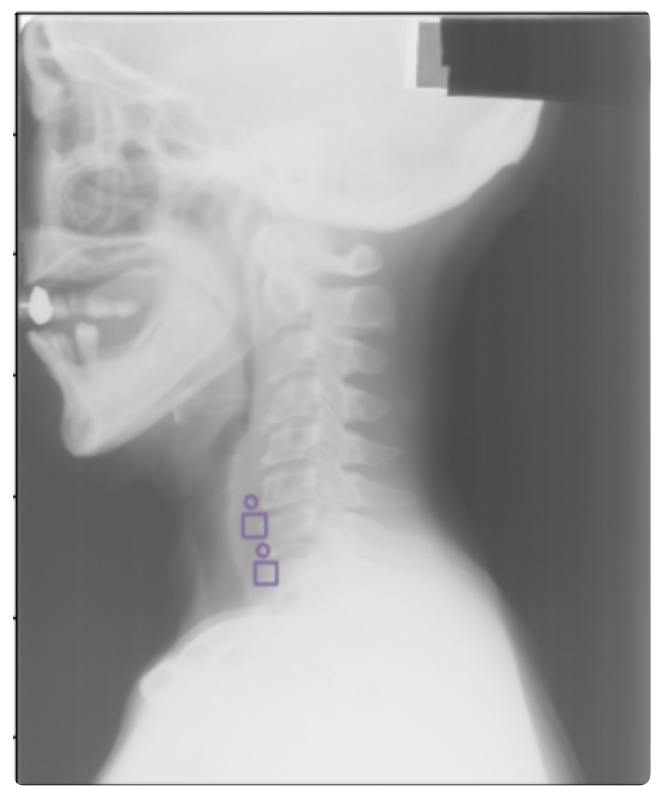
\includegraphics[width=0.25\textwidth]{Det_Result.png}
    \caption{Visualisation of poor performance from off-the-shelf detector - FasterRCNN. Purple circles denote annotation location and squares denote predicted bounding box.}
    \label{fig:detection-results}
\end{figure} %C00681 & C03453

\subsubsection{Patch size variability in SegPatch} 
While tiling produces a uniform patch size, SegPatch generates non-uniformly sized patches which may lead to lower resolution patches for the larger patches generated. 
Uniform patch size was not feasible as that either resulted in multiple missing osteophytes or a large number (and area) of overlaps between the patches. 
%The tiling approach was inspired from \cite{ozge2019power}, where the authors used it for a detection task of pedestrians and vehicles onboard a micro aerial vehicle (MAV) with high-resolution imagery.

% \subsection{Utilisation of non-annotated images}
% \label{Pretext-Problem}
% As there were 16627 non-annotated images, a pretext task using ResNet18 \cite{he2015deep}, comprising of a binary classification problem between the cervical and the lumbar view was posed. These weights (will be referred to as \textit{custom-weights} in the paper) were utilised to compare against imagenet weights in the identification tasks.

% \subsubsection{Potential problem in pretext task}
% \update{The use of custom weights deteriorated the performance for all sizes to nearly 0 in the case of detection. For patch-classification, for both methods, there was no visible improvement using the custom-weights.} 

% The pretext garnered 100\% validation accuracy and precision within 1 epoch. We hypothesize that this led to the weights not containing enough information about the images themselves. Future studies should definitely incorporate more complex pretext tasks such as those mentioned in \cite{albelwi2022survey} to potentially extract more information. Lastly, we could neither consider the non-annotated images healthy nor utilise them for additional osteophyte locations.

\subsection{Poor Performance from off-the-shelf detectors}
\label{detection}
%Initially, to account for the pixel location annotations as opposed to smaller area wide annotations, a detection style task was adopted. Therefore, alongside classification, a direct detection based approach was performed as well. The bounding boxes were created in a similar fashion to that of Falk et al \cite{falk2019u}. 
 Initially, to develop a solution for osteophyte detection, we investigated the state-of-the-art detection method, FasterRCNN \cite{girshick2014rich}, and achieved an average mAP and accuracy score of 0.1\%, 0.2\%, 20\% and 30\% as the size of the bounding increasing from 10, 18, 36 to 54 pixels, respectively.
 The results did not improve with different forms of augmentation (including tiling, which is originally devised for detection-based tasks) or utilizing the latest versions of YOLO (NAS, v8). The key positive insight derived from the detection task using FasterRCNN is seen in Fig. \ref{fig:detection-results}. The model clearly understands the typical locations where the osteophytes appear.
 Notably at the corners of the vertebrae. A trend similarly observed in VinDr-SpineXR study \cite{nguyen2021vindr}. Consequently, it is advisable for future methodologies to place greater emphasis on the identification aspect rather than localization in the context of osteophyte detection.

\begin{figure}
    \centering
    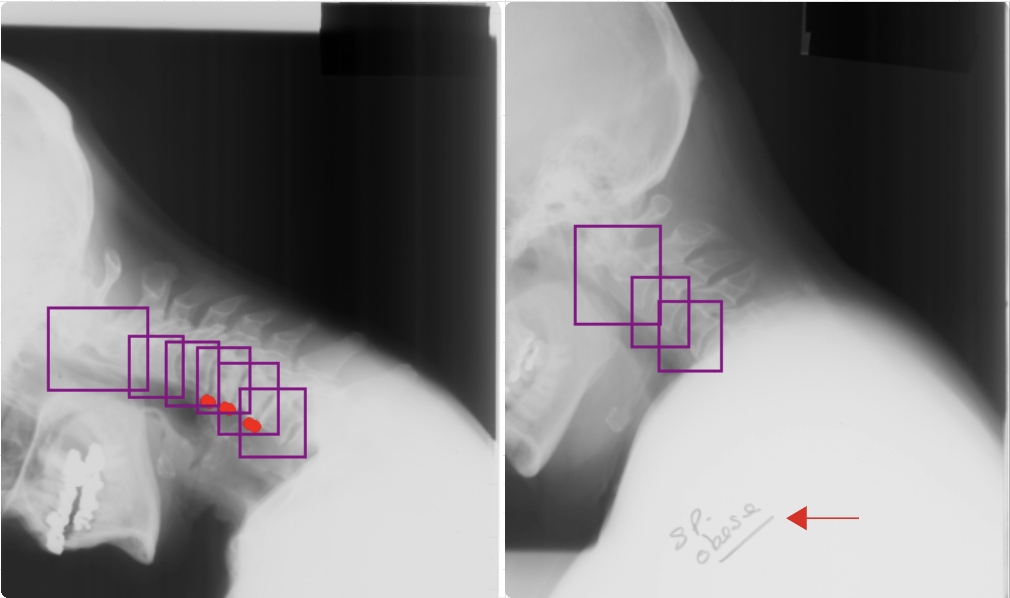
\includegraphics[width=0.32\textwidth]{images/Curvature.png}
    \caption{Example of difficult (but successful) to label scans. (Left): High curvature of spine. (Right): Presence of artifact  (text) denoted by red arrow with  with no osteophyte labels.}
    \label{fig:difficult}
\end{figure}

\section{Conclusion}
%%% Soumya: Completely rephrased the conclusion

% This work presents one of the first efforts towards the identification of spinal osteophytes. It combines a custom patching strategy SegPatch and a fine-tuned DenseNet-121 network. By classifying the patch, the identification procedure will become more efficient in both locating and identifying the osteophytes \soumya{as they generally tend to occur on the corners of the vertebrae.} \update{With 84\% metric scores for the patch classifier associated with well interpretable saliency maps,} this work not only paves way for a more efficient clinical approach to identifying osteophytes in X-rays, but also a standard pipeline towards medical key-point detection problems.
% \soumya{The study also highlights that detailed annotations may not be necessary for deep learning models to acquire meaningful insights. Presenting annotations as points, rather than generating complete masks or outlines, proved to be an efficient approach, leading to substantial time savings in the annotation process.}

This paper presents one of the first studies for spinal osteophyte detection. It integrates the use of a specialized patching strategy called SegPatch in conjunction with a fine-tuned DenseNet-121 network. By employing patch classification, the identification process gains enhanced efficiency in detecting osteophytes as osteophytes tend to generally originate in the corner regions of vertebrae. Our method achieves 84.5\% accuracy score and a 86.62\% specificity score for the patch classifier which generates saliency maps that align well with both positive and negative classifications. A study done by Nevalainen et al., showed a specificity of 75\% in detecting osteophytes from MRI \cite{nevalainen2023ultrasound}. 

The findings, combined with the analysis of the results in this paper lay the groundwork for a more effective clinical approach to osteophyte detection in X-ray images and other smaller structures. 
% medical key-point detection challenges.
\final{This is all while being robust to multiple orientations of the spine present in the scans, artifacts, minimal annotations and comparatively small training data.}

% In addition, this research presents that detailed annotations might not be imperative for deep learning models to derive significant insights in the case of medical keypoint detection. Instead of generating comprehensive masks, representing annotations as points proved to be a highly efficient approach, which can result into substantial time savings during the annotation process.
In addition, this work shows that osteophytes can be detected using a single modality instead of multi-modality approaches \cite{wang2016detection}.
% This advancement in spinal osteophyte identification can significantly benefit clinicians by streamlining the diagnostic process and providing a more efficient tool for detecting and characterizing osteophytes, all while working with X-ray images. 
This efficiency not only saves valuable time but also has the potential to enhance the accuracy and consistency of diagnoses, ultimately improving patient care and treatment outcomes.

% \section{Ethical Compliance}
% This research study was conducted retrospectively using human subject data made available in open access$^2$. Ethical approval was not required as confirmed by the license attached with the open access data.

% \subsection{Ethical Compliance}
% This research study was conducted retrospectively using human subject data made available in open access$^2$. Ethical approval was not required as confirmed by the license attached with the open access data.

\printendnotes


\subsection*{Acknowledgments}
S. S. Kundu was supported by the UK Medical Research Council
[MR/N013700/1] and the King’s College London MRC Doctoral Training Partnership
in Biomedical Sciences. Y. Mo is supported by the Oxford BDI-Novartis collaboration for AI in medicine. B. W. Papiez acknowledges Senior Fellowship at Population Health. The computational aspects of this research were supported by the Wellcome
Trust Core Award Grant Number 203141 /Z/16/Z and the NIHR Oxford BRC. The authors would also like to thank Mona Furukawa for her edits on the final manuscript.
%% Anissa helped me quite a bit with just running the cluster. Is there anyway I can mention this here?

% \theendnotes


% \label{sec:acknowledgments}


\bibliographystyle{IEEEbib}
\bibliography{ref}

\end{document}